\documentclass{article}\usepackage[]{graphicx}\usepackage[]{color}
%% maxwidth is the original width if it is less than linewidth
%% otherwise use linewidth (to make sure the graphics do not exceed the margin)
\makeatletter
\def\maxwidth{ %
  \ifdim\Gin@nat@width>\linewidth
    \linewidth
  \else
    \Gin@nat@width
  \fi
}
\makeatother

\usepackage{Sweavel}



\begin{document}



\begin{figure}
\begin{Schunk}


\centerline{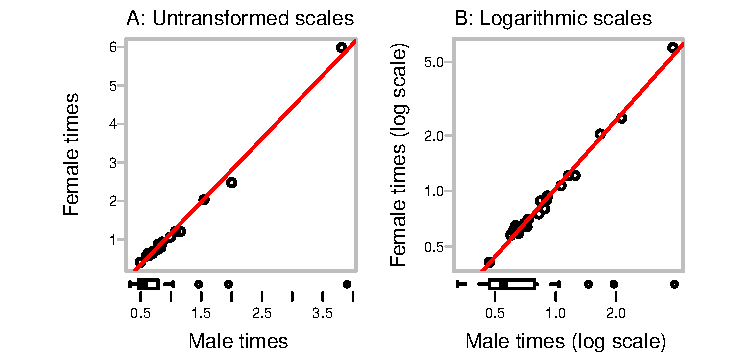
\includegraphics[width=\textwidth]{figs/11-fVSmTimeAB-1} }

\end{Schunk}
  \caption{Graphs compare female with male record times,
  for Northern Ireland hill races.  Least squares lines
    are added, and marginal boxplots are shown on the
    horizontal axis. Panel A
    has untransformed scales, while Panel B has log
    transformed scales.}\label{fig:nimff}
% \setfloatalignment{t}% forces caption to be top-aligned
\end{figure}




\end{document}
